\documentclass[11pt]{article}
\usepackage{arxiv}
\usepackage{amsmath,amssymb,booktabs,graphicx,hyperref,xcolor}
\usepackage{enumitem}
\hypersetup{pdfauthor={Ryan Gomez},colorlinks=true,linkcolor=black,citecolor=blue,urlcolor=blue}
\graphicspath{{generated/}{figures/}}
\renewcommand{\shorttitle}{Composition-only band-gap prediction}
\renewcommand{\headeright}{Development research}
\renewcommand{\undertitle}{A reproducible empirical study}
% Generated; do not edit numerical values.
\newcommand{\VOneMAE}{0.481}
\newcommand{\VOneRidge}{0.813}
\newcommand{\VTwoMAE}{0.976}
\newcommand{\VThreeMedian}{0.426}
\newcommand{\VThreeMean}{0.474}
\newcommand{\VThreeRidge}{0.815}
\newcommand{\VThreeDisposition}{SUPPORTED}
\newcommand{\VThreeDelta}{-0.048}
\newcommand{\VThreeLow}{-0.054}
\newcommand{\VThreeHigh}{-0.043}
\newcommand{\VThreeSeconds}{424.3}
\newcommand{\VThreeRSS}{372.9}
\newcommand{\VThreeMedianRMSE}{0.901}
\newcommand{\VThreeMeanRMSE}{0.875}
\newcommand{\VThreeUnits}{4601}

\title{Robust Tree Aggregation, Calibration, and Retrospective Selection for Experimental Band-Gap Prediction}
\author{Ryan Gomez}
\date{21 October 2026}
\begin{document}
\maketitle
\begin{abstract}
Composition-only band-gap models can screen historical materials cheaply, but low average error does not establish uncertainty calibration under chemical shift or prospective discovery. We report an auditable sequence of bounded CPU experiments on Matbench experimental inorganic band gaps. A preserved official-split development study attained mean absolute error (MAE) \VOneMAE{} eV versus \VOneRidge{} eV for ridge. Its uncertainty-weighted fixed-pool ranking showed retrospective utility, while element holdouts exposed substantial miscalibration. A direct-quantile successor collapsed to zero predictions, with MAE \VTwoMAE{} eV; a synthetic diagnostic identifies a constant-initial-gradient failure mechanism. We then froze a separate robust-aggregation study on \VThreeUnits{} canonical compositions, using three grouped five-fold repetitions, identical-tree mean/median controls, stronger classical baselines, representation and ensemble-size ablations, conformal residual calibration, ranking controls, and five element holdouts. Mean and median tree aggregation attained mean MAE \VThreeMean{} and \VThreeMedian{} eV, respectively. Their paired difference was \VThreeDelta{} eV, with an exploratory fixed-model bootstrap interval [\VThreeLow{}, \VThreeHigh{}] eV. The prespecified aggregation disposition is \VThreeDisposition{}. All data were previously inspected; these are development findings, not protected confirmation. No result establishes state-of-the-art performance, independent replication, stability, synthesizability, or discovery of a new material.
\end{abstract}
\keywords{materials informatics \and experimental band gap \and robust aggregation \and uncertainty \and reproducibility}

\section{Introduction}
Experimental band gaps influence how materials absorb and transport electronic excitations, but a band gap alone does not establish suitability for photovoltaics, catalysis, or a device. A composition-only predictor has a narrower purpose: provide a low-cost estimate when crystal structures and further measurements are unavailable. Such a predictor cannot distinguish polymorphs sharing the same formula, and its ranking must be interpreted as a screening heuristic rather than an experimental conclusion.

The Matbench experimental-gap task provides a standardized setting for this problem \cite{dunn2020matbench,zhuo2018bandgaps}. Yet a single pooled error can obscure the target's large zero-gap mass, unreliable uncertainty under element shifts, and weak comparisons against constant or linear baselines. A method can improve average prediction and still fail the scientific use case implied by its uncertainty estimates.

Our initial ExtraTrees study provided positive development evidence for prediction and historical ranking, alongside negative shift findings. A separately frozen quantile-boosting study then failed to learn useful point predictions. These outcomes motivate a precise successor question: \emph{does replacing the mean of a fixed ensemble's tree predictions with its median improve absolute error, without attributing extra training, information, or tuning to aggregation?} The mechanism predicts reduced sensitivity to a minority of large tree predictions in a zero-heavy target setting. It also predicts possible losses in squared error, positive-gap strata, or selection utility.

This paper's contribution is an empirical audit with a complete evidence chain, not a new tree-learning or conformal algorithm. We retain all predecessor outcomes, freeze one bounded successor, separate official and grouped evaluation, use identical-tree controls, and recompute important results from raw predictions using a verifier independent of the training metric implementation. The project reaches a defensible bounded conclusion even when some mechanisms fail.

\section{Related work and novelty boundary}
Composition-based gap prediction predates this study \cite{zhuo2018bandgaps}. Matbench standardizes datasets, outer folds, and reporting so that prediction methods can be compared consistently \cite{dunn2020matbench}. Our historical official-split evaluation preserves those rows and identifiers; our group-mean successor changes the experimental unit and is explicitly not a leaderboard submission.

Roost learns stoichiometric representations using element interactions, while CrabNet applies attention to composition representations \cite{goodall2020roost,wang2021crabnet}. These methods show why a hand-designed composition feature vector and a ridge comparison cannot support a state-of-the-art claim. We add stronger classical controls within our CPU budget, but do not substitute literature numbers for matched neural runs or claim those models have been defeated.

MODNet and a task-specific Bayesian optimization of CrabNet are stronger direct comparators. The latter reported official-fold MAE 0.3310 eV after nested hyperparameter search, while its comparison reported 0.3470 eV for MODNet \cite{debreuck2021modnet,baird2022saasbo}. Those official-task numbers are not directly comparable to our group-mean successor, and neither neural system was independently reproduced here. Redundancy-control work further shows that random splitting can overstate extrapolative performance \cite{li2024mdhit}. Our canonical grouping removes exact-equivalent overlap only; it does not establish generalization under broader chemical-distance control.

Extremely randomized trees are established nonlinear ensembles \cite{geurts2006extratrees}. Random forests and quantile regression forests likewise predate this work. Quantile regression forests use within-leaf response distributions \cite{meinshausen2006qrf}; the median of our tree \emph{leaf means} is a different estimator. We do not claim it is a consistent conditional-quantile estimator. The isolated contribution is the measured effect of aggregation in this task and resource regime.

Split conformal prediction provides marginal coverage under appropriate exchangeability and score-fitting assumptions \cite{lei2018conformal}. Conformalized quantile regression combines quantile estimation and calibration \cite{romano2019cqr}. Neither theorem guarantees coverage under arbitrary element holdout. Ensemble dispersion, a Gaussian ranking score, an empirical fraction of tree predictions, and a calibrated response distribution are distinct objects. We retain this distinction throughout.

\section{Data, units, and protected-evaluation boundary}
The pinned Matbench v0.1 \texttt{matbench\_expt\_gap} artifact contains 4,604 composition/experimental-gap rows. Inputs are formula-derived features; the target is measured gap in eV. No structures, relaxed geometries, computed properties, source-paper identifiers, or post-synthesis descriptors enter a model. The upstream source-data landing page declares MIT licensing, recorded in the data contract. Exact source bytes, metadata and outer splits are SHA-256-bound.

A scale- and order-invariant parser identifies 4,601 canonical compositions. Three pairs have conflicting recorded targets; their spans are 0.58, 0.64 and 2.30 eV. Two canonical groups cross official training/test boundaries in four folds. Historical v1 and v2 retain the original rows for comparability. The successor uses one unit per canonical composition, retaining all source IDs and labels and assigning the arithmetic mean of recorded gaps as its target. This explicit aggregation does not resolve measurement or polymorph ambiguity. It changes the task relative to the official benchmark, so cross-version absolute scores cannot isolate method improvement.

The historical dataset contains 2,450 exact zero labels. We retain them and separately evaluate zero and positive-target strata. We neither remove hard examples nor silently replace zero labels with missing values. The target is nonnegative, but model intervals are not clipped at zero; this preserves the declared interval construction.

All original labels and outcomes had been inspected before this successor. New group partitions therefore remain \textbf{development evaluations}. There is no protected external test set, prospective synthesis, or independently operated replication in this evidence package. Group isolation repairs a particular overlap problem; it cannot undo adaptive knowledge of the benchmark.

\section{Full model specification}
\begin{figure}[htbp]\centering
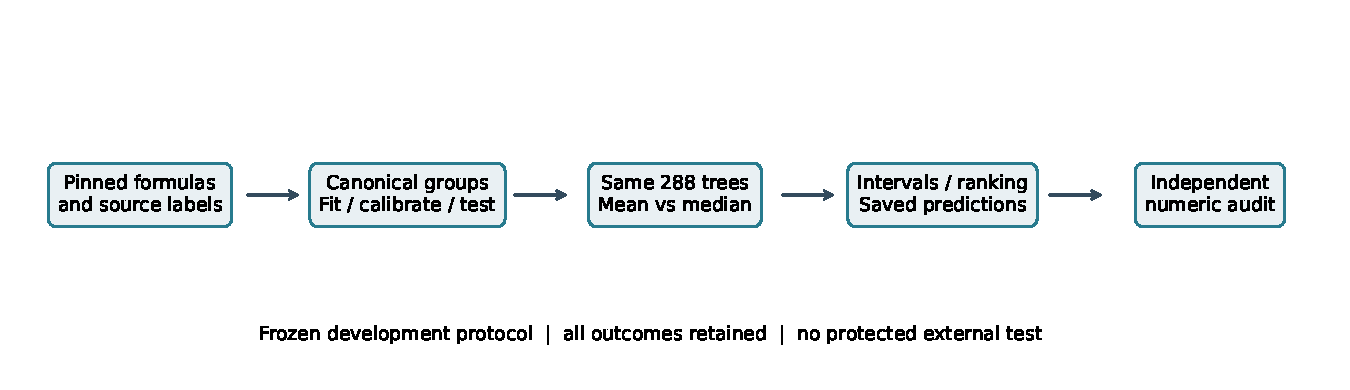
\includegraphics[width=\linewidth]{workflow.pdf}
\caption{Execution and evidence flow. Labels are excluded from feature construction and ranking decisions; calibration labels are used only by the declared interval construction.}
\end{figure}
\subsection{Formula representation}
A parser maps a formula to element fractions $x_e\geq0$, $\sum_e x_e=1$, over 118 elements. The fixed 128-dimensional vector consists of those fractions and ten descriptors: element count, fraction entropy $-\sum_e x_e\log x_e$, minimum and maximum nonzero fraction, $\ell_2$ norm of fractions, and weighted mean, weighted standard deviation, minimum, maximum and range of atomic number. No descriptor depends on target values. A train-only occurrence count records unseen elements for inference reporting; it does not change the fixed feature matrix. Fractions and aggregate features are stored as float32. Equivalent scaled, reordered and parenthesized formulas must give identical features.

\subsection{Shared tree learner and aggregation}
Each of three seeds, 7, 17 and 29, fits 96 ExtraTrees regressors with maximum depth 22, minimum leaf size two, feature fraction 0.7, no bootstrap, squared-error splits, and one worker. The ensemble therefore has $T=288$ tree predictions. For a query $x$, write $a_t(x)$ for tree $t$'s leaf mean. The matched predictions are
\begin{equation}
 f_{\rm mean}(x)=\frac{1}{T}\sum_{t=1}^{T}a_t(x),\qquad
 f_{\rm med}(x)=\operatorname{median}_{t=1}^{T}a_t(x).
\end{equation}
The median for even $T$ averages the central pair. Both methods use exactly the same fitted trees and rows. There is no extra optimization, parameter fitting or target access for the median. It can suppress a minority of high predictions, but does not generally equal $\operatorname{median}(Y\mid X=x)$. This distinction is a falsifiable limitation, not an unproved consistency claim.

The first-seed 96-tree median is an ensemble-size ablation; another 288-tree ensemble uses only the 118 element fractions. Tree count is matched for that feature ablation. Tree predictions are cast to float32 before aggregation, with float64 means, standard deviations and median calculations. Checkpoints store the featurizer, exact feature names, models, calibration scores, fit/calibration keys, and configuration digest. Reloaded tree predictions must be exactly equal before a cell is accepted.

\subsection{Intervals and their assumptions}
Proper-training trees produce a dispersion score
\begin{equation}
 s(x)=\max\left\{0.05\ \mathrm{eV},\;\sqrt{\frac{1}{T-1}\sum_t(a_t(x)-f_{\rm mean}(x))^2}\right\}.
\end{equation}
The floor is fixed before successor execution. For an aggregation $m\in\{\mathrm{mean},\mathrm{med}\}$ and $n_c$ calibration units, define $r_i=|y_i-f_m(x_i)|/s(x_i)$. At nominal coverage $c$, let $k=\lceil(n_c+1)c\rceil$ and $q_c$ be the $k$th ordered score, with $q_c=+\infty$ if $k>n_c$. The interval is
\begin{equation}
 I_c(x)=[f_m(x)-q_cs(x),\;f_m(x)+q_cs(x)].
\end{equation}
A constant-width control replaces $s$ by one. All interval variants reuse the same training and calibration partition. We report 50, 80, 90 and 95\% coverage, width, and the proper interval score
\begin{equation}
 S_\alpha(l,u;y)=(u-l)+\frac{2}{\alpha}(l-y)_++\frac{2}{\alpha}(y-u)_+,\quad \alpha=1-c.
\end{equation}
The usual rank argument applies conditionally on fitted training state only when the calibration and query scores are exchangeable: a query rank is uniform among $n_c+1$ positions, up to ties, giving the corresponding marginal lower coverage bound. We invoke no claim of exchangeability for the chemical holdouts or representative sampling of all possible materials. Historical v1 fitted its floor on calibration inputs and clipped the small-sample rank; its observed coverage is retained, but it does not inherit the corrected successor construction retroactively. A common multiplicative scale cancels normalized interval widths, while its use in Gaussian ranking still does not establish a probability model.

\subsection{Label-blind ranking}
For the fixed window $W=[1.1,1.6]$ eV, four policies operate on saved out-of-fold predictions. Empirical tree mass is $T^{-1}\sum_t\mathbf1\{a_t(x)\in W\}$. The Gaussian working score is $\Phi((1.6-f_{\rm med}(x))/s(x))-\Phi((1.1-f_{\rm med}(x))/s(x))$. Greedy ranking orders by $-|f_{\rm med}(x)-1.35|$. Random selection uses 64 deterministic permutations. The first two scores are heuristics, not certified probabilities. Stable canonical-order tie breaking is explicit. Labels are read only for evaluation after order is fixed. Budgets are 10, 25, 50 and 100, with hits, precision and enrichment against pool prevalence retained for every repeat.

\subsection{Training, inference and complexity}
Training chronologically validates source hashes, forms canonical units, freezes split membership, fits training-only feature state, fits models, scores calibration units, scores outer-test units, serializes and reloads the shared ensemble, then evaluates and records outcomes. Baselines and ablations run sequentially to avoid keeping several large forests resident. The original model is deleted before checkpoint reload. Inference parses a formula, applies the saved featurizer, evaluates all trees, takes the median, and applies saved calibration scores. An unseen-element flag reports support limitations; it does not supply an OOD guarantee.

Typical tree construction scales roughly as $O(Tdn\log n)$ for balanced trees with $d$ candidate features, with implementation- and data-dependent depth. Prediction is $O(TD)$ per query at depth $D\leq22$. Memory includes tree nodes, the $n\times128$ feature matrix, and query-by-tree prediction matrices. These are descriptive orders, not measured speedup claims. Actual node counts, elapsed time, resource peaks, and artifact sizes are retained.

\section{Experimental design and fixed stopping rules}
\subsection{Grouped repetitions and controls}
For seeds 20261021, 20261022 and 20261023, canonical keys are ordered by SHA-256 of \texttt{seed:canonical}, then assigned round-robin to five folds. Each outer training pool is hash-ordered with seed plus 731; the first rounded 20\% becomes calibration and the remainder proper training. Every fit, calibration and test set is nonempty, disjoint and exhaustive. All baseline fitting uses the same proper-training rows.

Controls are: the exact-tree mean, a 288-tree random forest with bootstrap and otherwise matched depth/leaf/feature settings, histogram gradient boosting with 160 iterations, learning rate 0.05, 31 leaves, minimum leaf 20, squared-error loss and no early stopping, standardized ridge with training-only RidgeCV over $10^{-3},10^{-2},10^{-1},1,10,100$, and the proper-training median. Random forest and ExtraTrees have matched tree budgets, not guaranteed equal time or parameter count. All thread counts are one. Neural baselines, structure models and external datasets are not part of the bounded empirical claim.

\subsection{Endpoints and decision rule}
The primary endpoint is pooled out-of-fold MAE difference $\Delta_r=\mathrm{MAE}_{\rm median,r}-\mathrm{MAE}_{\rm mean,r}$ for each repetition. Before execution, support required $\Delta_r\leq-0.01$ eV for \emph{every} repetition. All nonnegative differences imply NEGATIVE; remaining outcomes are MIXED. The scientific result must not be selected by whichever model or endpoint wins after inspection.

Secondary results include RMSE, $R^2$, Spearman correlation, interval coverage/width/score, ranking, and zero/positive/oxygen/conflicting-duplicate strata. We report all models and repeats. These secondary endpoints receive no confirmatory significance claim or selective multiplicity interpretation.

An exploratory bootstrap averages each canonical unit's paired absolute-error difference across repeats, then resamples canonical units 5,000 times with seed 20261021. The percentile interval conditions on fitted models. It does not include full retraining uncertainty or treat overlapping CV folds as independent experiments. It therefore cannot convert development evidence into a confirmatory result.

\subsection{Ablations, robustness and chemical shift}
Representation and ensemble-size ablations use all outer cells. First-repeat/fold-zero probes use 96 trees and fixed 25\% and 50\% proper-training subsets, 0.1 eV Gaussian label noise, and a label permutation. Their scope is an exploratory diagnostic, not a full learning-curve or robustness theorem. Li, Zn, Ga, Se and Te holdouts remove all compositions containing the named element from training and calibration. Mean and median aggregation share their fitted ensemble. Every holdout prediction and interval is saved.

A synthetic fixture contains 200 ordered inputs, 60\% with zero response and 40\% with a deterministic positive response. Quantile boosting at $\tau=0.5$ compares default median initialization with a positive constant initialization using otherwise identical settings. Initial gradients, first-tree nodes, distinct outputs and fixture training error diagnose optimization behavior. This is not a post-hoc replacement for the frozen negative v2 benchmark.

\subsection{Compute contract and failure preservation}
One new scientific configuration was authorized, with at most three hosted attempts for genuine infrastructure repairs, a one-hour CPU limit per attempt, maximum process RSS 512 MiB, and no rising pageouts. Resource-monitor absence fails closed. The main matrix begins only after software tests and a synthetic end-to-end run. No tree count, split, seed, metric or threshold may be changed to rescue an observed score. Historical failed runs, tracebacks and checkpoints remain intact. Failed or partial cells cannot be pooled into a successful result.

\section{Results}
\subsection{Preserved official-split study}
\begin{table}[htbp]\centering\small
\caption{Historical official-split results (v1); canonical duplicates are retained.}
\begin{tabular}{lrr}
\toprule
Model & MAE (eV) & RMSE (eV) \\
\midrule
ExtraTrees mean & 0.481 & 0.906 \\
Ridge & 0.813 & 1.161 \\
Training median & 0.976 & 1.744 \\
\bottomrule
\end{tabular}\end{table}

The historical ExtraTrees mean attained \VOneMAE{} eV MAE against \VOneRidge{} eV for ridge. An independent standard-library audit recomputed MAE and RMSE from saved predictions, checked all 4,604 original labels and official fold IDs, verified file hashes and resource receipts, and reproduced the saved values. This verifies the recorded calculation, not an independently trained replication.

The historical candidate policy selected 38 target-window hits at budget 50, versus 15 for greedy ranking and mean 3.58 for 64 random selections. These remain retrospective development results. Historical nominal 90\% coverage was 0.889, with 1.604 eV mean width, but selenium-holdout coverage fell to 0.525. The original holdout reports are aggregate-only; the successor addresses this provenance gap with row-level artifacts.

\subsection{Grouped aggregation and baseline comparison}
\begin{table}[htbp]\centering\small
\caption{Grouped development MAE in eV. Repetitions share the same canonical units and are not independent datasets.}
\begin{tabular}{lrrrr}
\toprule
Model & Repeat 1 & Repeat 2 & Repeat 3 & Mean MAE \\
\midrule
ExtraTrees mean & 0.476 & 0.475 & 0.470 & 0.474 \\
ExtraTrees median & 0.429 & 0.428 & 0.419 & 0.426 \\
Median, 96 trees & 0.431 & 0.428 & 0.422 & 0.427 \\
Median, fractions only & 0.546 & 0.546 & 0.536 & 0.543 \\
Random forest & 0.520 & 0.521 & 0.519 & 0.520 \\
Histogram boosting & 0.555 & 0.547 & 0.544 & 0.549 \\
Ridge & 0.814 & 0.815 & 0.816 & 0.815 \\
Training median & 0.976 & 0.976 & 0.976 & 0.976 \\
\bottomrule
\end{tabular}\end{table}

The grouped successor's prespecified aggregation disposition is \textbf{\VThreeDisposition{}}. The mean paired effect was \VThreeDelta{} eV, with exploratory fixed-model interval [\VThreeLow{}, \VThreeHigh{}] eV. This effect compares identical tree sets within each cell and therefore cannot be explained by extra training data, more trees, a different optimizer or additional model-selection trials. It can still depend on this dataset's zero-heavy distribution and on the chosen tree learner. Absolute scores must not be compared to v1 as though the evaluation units and splits were identical.
\begin{figure}[htbp]\centering
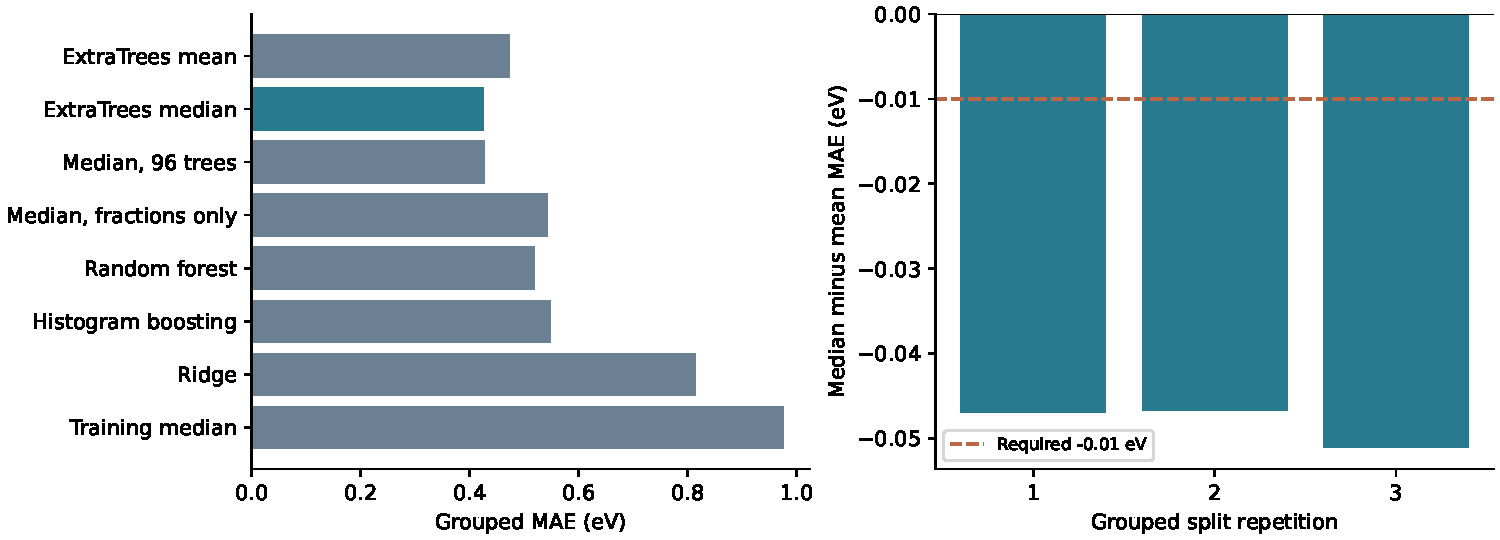
\includegraphics[width=\linewidth]{aggregation.pdf}
\caption{Grouped baseline errors and paired aggregation effects. The dashed line marks the preregistered development threshold, not a fitted optimum. All three repetitions are displayed.}
\end{figure}
\begin{table}[htbp]\centering\small
\caption{Subgroup absolute error in eV, averaged across repeats. Subgroups overlap; the three conflicting duplicate units are too few for stable inference.}
\begin{tabular}{lrrr}
\toprule
Stratum & Units & Mean aggregation MAE & Median aggregation MAE \\
\midrule
zero & 2449 & 0.331 & 0.228 \\
positive & 2152 & 0.636 & 0.651 \\
contains\_oxygen & 1090 & 0.799 & 0.712 \\
conflicting\_duplicates & 3 & 0.445 & 0.541 \\
\bottomrule
\end{tabular}\end{table}

The improvement is not uniform. Median aggregation increases average RMSE from
\VThreeMeanRMSE{} to \VThreeMedianRMSE{} eV and increases positive-gap MAE in
every repetition. Its overall MAE gain is driven by the zero-gap stratum.
The 96-tree ablation is close to the full median ensemble, while removing the
ten aggregate descriptors substantially degrades MAE. These findings constrain
the mechanism: neither universal error reduction nor a large ensemble-size
advantage is established.

\subsection{Uncertainty and shift}
\begin{table}[htbp]\centering\small
\caption{Mean across three repeats at nominal 90\% coverage; normalized and constant-width residual calibration use the same proper-training models.}
\begin{tabular}{lrrr}
\toprule
Method & Coverage & Width (eV) & Interval score \\
\midrule
mean constant & 0.903 & 2.690 & 4.467 \\
mean normalized & 0.906 & 1.764 & 3.033 \\
median constant & 0.904 & 2.699 & 4.728 \\
median normalized & 0.907 & 1.893 & 3.244 \\
\bottomrule
\end{tabular}\end{table}

\begin{table}[htbp]\centering\small
\caption{Element-holdout development results. Intervals target nominal 90\% coverage; exchangeability is not assumed under these shifts.}
\begin{tabular}{lrrrr}
\toprule
Element & Aggregation & MAE (eV) & Coverage & Width (eV) \\
\midrule
Li & mean & 1.036 & 0.931 & 3.833 \\
Li & median & 0.670 & 0.913 & 4.086 \\
Zn & mean & 0.505 & 0.822 & 1.598 \\
Zn & median & 0.489 & 0.822 & 1.657 \\
Ga & mean & 0.602 & 0.771 & 1.569 \\
Ga & median & 0.609 & 0.776 & 1.747 \\
Se & mean & 0.967 & 0.530 & 1.695 \\
Se & median & 1.016 & 0.518 & 1.795 \\
Te & mean & 0.675 & 0.691 & 1.611 \\
Te & median & 0.717 & 0.667 & 1.762 \\
\bottomrule
\end{tabular}\end{table}

\begin{figure}[htbp]\centering
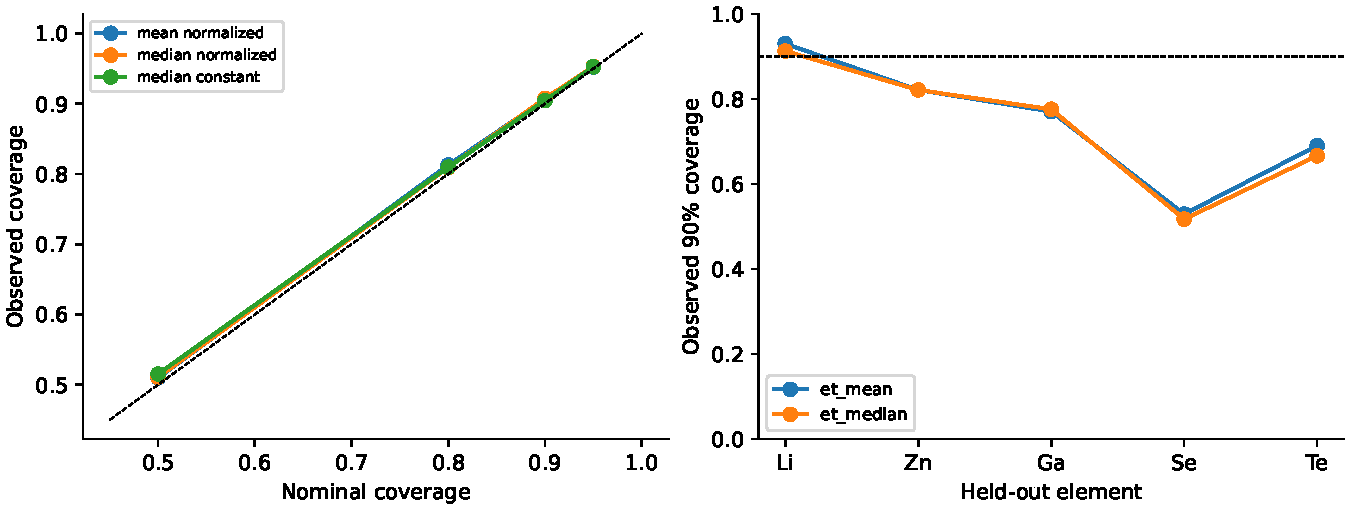
\includegraphics[width=.94\linewidth]{calibration_shift.pdf}
\caption{Marginal calibration and element-shift coverage. A nominal level is a target under assumptions, not a promise under arbitrary chemical shift.}
\end{figure}
Coverage and width must be considered together. An interval that over-covers by being very wide does not establish sharp predictive uncertainty. Conditional and OOD failures remain scientifically material even if average marginal calibration is acceptable.

\subsection{Ranking, ablations and probes}
\begin{table}[htbp]\centering\small
\caption{Retrospective candidate selection at budget 50, averaged across repetitions. Probability-like scores are working heuristics.}
\begin{tabular}{lrrr}
\toprule
Policy & Mean hits / 50 & Precision & Enrichment \\
\midrule
empirical tree mass & 36.333 & 0.727 & 10.855 \\
gaussian working & 37.333 & 0.747 & 11.154 \\
greedy median & 20.333 & 0.407 & 6.075 \\
random & 3.578 & 0.072 & 1.069 \\
\bottomrule
\end{tabular}\end{table}

\begin{figure}[htbp]\centering
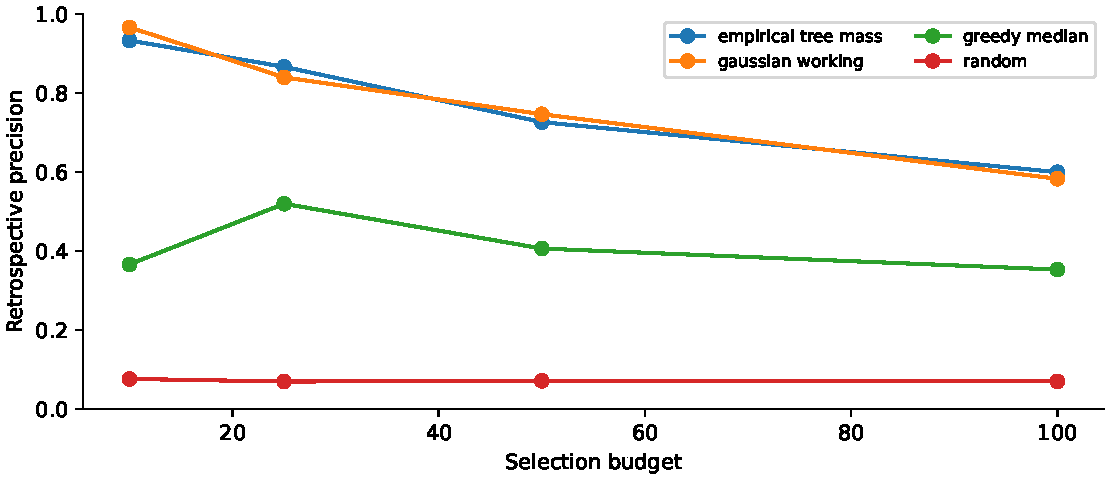
\includegraphics[width=.86\linewidth]{selection.pdf}
\caption{All predefined selection budgets. Curves average the same three split repetitions; they are not independent prospective campaigns.}
\end{figure}
\begin{table}[htbp]\centering\small
\caption{First-repeat, first-fold exploratory probes with 96 trees. These do not establish full scaling laws or general robustness.}
\begin{tabular}{lrrr}
\toprule
Probe & Fit units & MAE (eV) & RMSE (eV) \\
\midrule
scale 25 & 736 & 0.563 & 1.120 \\
scale 50 & 1472 & 0.491 & 0.975 \\
noise 0.1 & 2944 & 0.465 & 0.940 \\
permuted & 2944 & 1.125 & 1.436 \\
\bottomrule
\end{tabular}\end{table}

The representation and ensemble-size rows in the main comparison are matched ablations. Ranking compares working distributional heuristics against point-greedy and random controls at equal budgets. A selected formula is not a stable or synthesizable candidate by virtue of its predicted gap. Repeated fixed-pool scores do not constitute independent discovery campaigns.

\subsection{Negative quantile study and mechanism diagnostic}
The preserved direct-quantile v2 point model returned zero on every recorded row and attained \VTwoMAE{} eV MAE. Its 90\% intervals covered approximately 0.939 with mean width 2.749 eV; neither observation rescues its failed point-prediction objective.
\begin{table}[htbp]\centering\small
\caption{Synthetic zero-mass diagnostic; training errors on a hand-defined fixture are not benchmark performance.}
\begin{tabular}{lrrr}
\toprule
Initialization & First-tree nodes & Distinct outputs & Fixture MAE \\
\midrule
default median & 1 & 1 & 0.7206 \\
positive initialization & 3 & 23 & 0.0129 \\
\bottomrule
\end{tabular}\end{table}

At a mass point, the implemented pinball-loss subgradient can be identical across all training examples under zero initialization. A constant first pseudo-gradient offers no split signal; median leaf updates can remain zero. The synthetic counter-initialization demonstrates that this failure mode is compatible with learnable data. It does not establish that a changed initializer improves Matbench performance. Such a benchmark modification would require a separately frozen successor; none was used to rewrite v2.

\section{Efficiency and implementation verification}
\begin{table}[htbp]\centering\small
\caption{Measured outer-cell fit/prediction costs. Shared ExtraTrees timing includes calibration predictions; checkpoint I/O is outside that timer. Node counts are retained in the raw cost table.}
\begin{tabular}{lrrr}
\toprule
Model operation & Cells & Mean seconds & Max seconds \\
\midrule
fractions only & 15 & 4.612 & 4.700 \\
hist gradient boosting & 15 & 1.737 & 1.856 \\
random forest & 15 & 10.239 & 10.680 \\
ridge & 15 & 0.062 & 0.099 \\
shared extra trees & 15 & 5.801 & 5.879 \\
train median & 15 & 0.001 & 0.001 \\
\bottomrule
\end{tabular}\end{table}

The grouped successor completed in \VThreeSeconds{} seconds with peak observed process RSS \VThreeRSS{} MiB under the unchanged 512 MiB limit. The resource receipt records zero pageout increase. The runtime includes the declared models, ablations, holdouts, probes, checkpoint checks and output work; it is not inference latency or an equal-runtime comparison between architectures.

The software includes executable training and inference, typed configuration access, canonical parsing, exact split manifests, baselines, calibration, candidate ledgers, numerical safeguards, deterministic seeds, checkpoint serialization, failure retention and result generation. Tests include hand-verifiable aggregation and interval ranks, malformed inputs, formula invariance, split isolation, checkpoint behavior, corrupted-artifact refusal, metric correctness and bootstrap unit handling. The hosted synthetic end-to-end check exercises the same orchestrator at small scale before expensive fitting. Fixture success is engineering evidence only.

\section{Failure analysis and discussion}
Three lessons survive the audit. First, a favorable in-distribution score can coexist with poor chemical-shift uncertainty; model selection should not erase that conflict. Second, a negative quantile result may reflect initialization dynamics rather than absence of composition signal. Third, an aggregation claim is most cleanly tested by holding the fitted tree ensemble fixed. Adding architecture, descriptors or tuning simultaneously would obscure the mechanism.

The successor's terminal classification refers only to its predefined aggregation endpoint. Comparisons with random forest, boosting and ridge contextualize the result, but do not establish global optimality. Secondary tradeoffs, including positive-gap accuracy and ranking, remain part of the full result even if the primary endpoint is supported. The practical threshold and study budget were fixed before successor outcomes; further improvements are new hypotheses, not permission for indefinite positive-result search.

\section{Limitations and threats to validity}
\begin{enumerate}[leftmargin=*]
\item \textbf{Development reuse.} All labels were previously inspected. Repeated CV and post-hoc bootstrap cannot restore a protected confirmatory boundary.
\item \textbf{Composition ambiguity.} Polymorphs and measurement conditions are not identifiable. Averaging three conflicting groups is an explicit target convention, not a physical resolution.
\item \textbf{Selection and zero mass.} The benchmark is not a random sample of possible materials; its zero-gap population can dominate global metrics and easy abstention strata.
\item \textbf{Incomplete competitive scope.} Neural composition models, richer descriptors, structure models and external datasets were not run. No SOTA or broad superiority claim is made.
\item \textbf{Uncertainty assumptions.} Tree dispersion and probability-like ranking scores do not identify a true conditional density. Marginal calibration does not imply subgroup or OOD coverage.
\item \textbf{Dependent evaluation.} Training folds overlap, repetitions share units, and fixed-model bootstrap intervals omit retraining uncertainty.
\item \textbf{Retrospective utility.} Historical labels are revealed after ranking, but this is not a prospective sequential campaign, synthesis study, or device evaluation.
\item \textbf{Verification boundary.} Artifact recomputation, hosted execution, and software tests are not an independent scientific replication or independent implementation.
\end{enumerate}

\section{Reproducibility, evidence and release}
The canonical research state records question, budget, scope, claims, frozen predecessors and current disposition. Separate protocol files specify v1, v2 and v3. Raw source hashes, dataset metadata, canonical source-label mappings, per-cell split indices, source-file digests, dependency versions, tests, logs and resource receipts accompany the output. Historical failed experiments are retained rather than hidden.

The successful predecessor used Python 3.13.15, NumPy 2.1.3, scikit-learn 1.6.1, Matplotlib 3.10.0 and joblib 1.6.0 on Kaggle Linux. The v3 launcher checks the frozen core dependency versions, records the full relevant host versions, and sets numerical-library thread counts to one. The local lock is a distinct build environment and is not represented as identical to that runtime.

The independent numerical verifier uses only Python's standard library. It checks original target alignment, official or grouped fold membership, complete per-repeat predictions, model coverage, arithmetic scores, intervals, ranking order, holdout metrics, resource conditions and manifest bytes. It does not deserialize potentially untrusted model objects. Checkpoint loading is restricted to trusted project artifacts. Paper macros, comparison tables and plots are generated after verification; an evidence manifest maps output files to source runs and hashes.

A post-release adversarial audit found four summary-verification gaps: an altered primary mean, an omitted calibration matrix, a false ranking precision, and an incorrect completed-cell count could pass the earlier verifier after the associated file manifest was updated. The repaired verifier rejects all four corrupted copies; the untouched original outputs pass. It additionally verifies source-formula ratios, complete calibration/ranking/subgroup matrices and subgroup errors. A separate arithmetic implementation, using NumPy only for the specified random stream and percentile convention, exactly recomputes all 5,000 bootstrap replicates' resulting interval and all 12 random-ranking summaries. The updated release has 72 passing software tests. Original frozen execution code and historical receipts are preserved separately from these verification repairs.

\subsection{Fresh frozen-source computational reproduction}
\begin{table}[htbp]\centering\small
\caption{Identical frozen-source executions. Predictions, split files and all 20 checkpoints match byte for byte; both runs record zero pageout increase. Timing differences are environmental, not a model speedup.}
\begin{tabular}{lrrr}
\toprule
Execution & Cells & Seconds & Peak RSS (MiB) \\
\midrule
Original v3 & 20 & 424.3 & 372.9 \\
Fresh reproduction & 20 & 369.8 & 372.1 \\
\bottomrule
\end{tabular}\end{table}

One additional Kaggle execution used the exact original source transport, dataset, model settings, split seeds and resource guards under a new run identifier. Its saved predictions, canonical units, splits, diagnostic outputs and all 20 checkpoint files match the original byte for byte. All scientific summaries match exactly when declared timing fields are excluded. Both executions used matching recorded core numerical dependencies. This is a same-operator computational reproduction, not an independent implementation, independent scientific replication or protected external evaluation. Aggregate exploratory-probe results also reproduce, but their original row-level predictions were not retained; those probes therefore lack the direct row-level audit available for the primary and chemical-holdout results.

The source, final PDF, bibliography, unchanged recovered arXiv-style file, generated assets, frozen configurations, tests, scripts and distributable evidence form the reproducibility package. The GitHub snapshot is scoped to this project within the configured Atlas repository. This release is a development research artifact; it is not a model safety certification or an arXiv submission receipt.

\section{Conclusion}
The preserved official-split study establishes positive development prediction and retrospective ranking evidence, accompanied by substantial shift limitations. The direct-quantile successor is a retained negative result with a reproducible synthetic failure mechanism. The grouped identical-tree aggregation experiment reaches \textbf{\VThreeDisposition{}} under its predefined rule, with median and mean MAE \VThreeMedian{} and \VThreeMean{} eV. The bounded research question is answered by the complete evidence, rather than by a requirement that every endpoint improve. External validation, independently operated reproduction, and prospective materials discovery remain separate unanswered questions.

\appendix
\section{Exact executable procedure}
From the project root, use a clean environment satisfying the recorded hosted versions. The following commands are executable interfaces, not pseudocode:
\begin{verbatim}
python -m pytest -q
python scripts/dry_run_robust.py
python -m ml4materials run-robust --run-id UNIQUE_RUN_ID
python scripts/verify_evidence.py --run-id UNIQUE_RUN_ID
python -m scripts.verify_resampling --run-id UNIQUE_RUN_ID
python -m ml4materials predict-robust \
  --checkpoint runs/UNIQUE_RUN_ID/models/repeat_0_fold_0.joblib \
  --formula GaAs --formula ZnO
python -m scripts.generate_paper_assets --robust-run UNIQUE_RUN_ID
tectonic paper/main.tex
\end{verbatim}
An unused run ID is mandatory. Resource refusal is retained as a failed run and must not be bypassed. A clean local execution is computational reproduction; independent scientific replication additionally requires independently operated evaluation and critical review.

\section{Claim-to-evidence map}
\begin{center}\small
\begin{tabular}{p{.28\linewidth}p{.62\linewidth}}\toprule
Claim & Retained source artifact \\\midrule
Official point performance & v1 \texttt{predictions/oof\_predictions.csv}, original data and split contract \\
Aggregation effect and baselines & v3 \texttt{predictions/oof.csv}, \texttt{splits.json}, \texttt{tables/metrics.csv} \\
Interval behavior & v3 saved outer lower/upper bounds and \texttt{tables/calibration.csv} \\
Historical selection utility & v1 candidate ledger and ranking table \\
Grouped ranking & v3 \texttt{predictions/ranking.csv}, score columns, exact ranks and source labels \\
Chemical shift & v3 \texttt{predictions/holdouts.csv} and saved holdout checkpoints \\
Quantile collapse & v2 row predictions and v3 \texttt{quantile\_diagnostic.json} \\
Software and compute & hosted JUnit XML, step logs, source hashes, resource receipts \\
Exact reproduction & \texttt{artifacts/reproduction-comparison-20261021.json} \\
Adversarial verifier repair & \texttt{artifacts/adversarial-audit-20261021.json} \\
Paper values & \texttt{paper/generated/evidence-map.json} and generation script \\\bottomrule
\end{tabular}
\end{center}
No claim in this table supplies absent external experiments. A source hash proves byte identity, not scientific validity; numerical, methodological and interpretation checks are all required.

\clearpage
\bibliographystyle{plain}
\bibliography{references}
\end{document}
